A Half Wave Plate (HWP) is an optical device that introduces a phase delay between the two orthogonal polarizations of the incoming signal. It can be made of birifringent crystals (e.g. Sapphire) or metamaterials. The HWP flips the polarization of incoming light along the fast axis of the crystal resulting in a polarization shift of $2\chi$, where $\chi$ is the incoming polarization angle of the light with respect to the fast axis. Thus, a HWP rotating with frequency $f$ mo\-du\-la\-tes the incoming polarization at $2f$, which is detected in the bolometer timestreams at $4f$. The demodulation process described below summarizes the formalism defined in Kusaka \& Essinger-Hileman et al., 2014~\cite{ABS_HWP}.

The detector timestream $d_{m}$ is composed of the unpolarized sky intensity $I$, the modulated polarization signal $P(\chi)$, white noise $N_{w}$, and spurious modulation signals $A(\chi)$ that depend on the HWP angle $\chi$ such that
\begin{equation}
d_{m}= I + P(\chi)+ N_{w} + A(\chi).
\end{equation}
The modulated polarization signal can be represented in terms of the Stokes $Q$ and $U$ parameters, eq.~(\ref{eqn:Stokes})), as
\begin{equation}
P(\chi)=\epsilon \mathrm{Re}\{(Q+iU) m(\chi)\},
\end{equation}
where the modulation is given by $m(\chi)=\exp[-4 i \chi]$ and $\epsilon$ is the polarization modulation efficiency factor, which is close to one. The spurious modulation signals $A(\chi)$ consist of components at every harmonic $n$ of the HWP rotation frequency and can be decomposed into cosine and sine components as
\begin{equation}\label{eqn:achi}
A(\chi)= \sum_{n} A_n(\chi)=\sum_{n}\Big[ (A^{nc}_{0} + \lambda^{nc} I) \cos(n\chi) + (A^{ns}_{0} + \lambda^{ns} I) \sin(n\chi)    \Big].
\end{equation}
Here the $A_{0}$ terms are stable and independent of the sky intensity and the $\lambda$ terms are small~\cite{ABS_HWP}.

The demodulated timestream is, then, extracted by applying a bandpass filter to $d_{m}$ to account for the slight variations in $f$, multiplying $d_{m}$ by $m^*(\chi)$, and applying a low-pass filter that passes $f\lesssim2$~Hz to eliminate higher order terms and all $A^{nc,s}$ and $\lambda^{nc,s}$ terms other than the $n=4$ components. From~\cite{ABS_HWP}, the final demodulated timestream $d_{\bar{d}}$ is then given by
\begin{equation}
d_{\bar{d}}=\frac{1}{2}\Big(\epsilon Q + A^{4c}_{0} + \lambda^{4c} I \Big) + N^{\mathrm{Re}}_{w} + \frac{i}{2}\Big(\epsilon U + A^{4s}_{0} + \lambda^{4s} I \Big) + iN^{\mathrm{Im}}_{w}.
\end{equation}

The optical action of a single layer birifringent material or achromatic metamaterial HWP can be described by the Mueller matrix:
\begin{equation}
M=\begin{bmatrix}
   t  &\rho  &0  &0\\
   \rho  &t  &0  &0\\
   0  &0  &c  &-s\\
   0  &0  &s  &c
\end{bmatrix}.
\label{eq:Mueller_Matrix}
\end{equation}

The $t$ term is proportional to the total unpolarized intensity transmitted by the HWP, the $\rho$ term to the differential transmission of the HWP. The $c$ and $s$ terms are responsible for the modulation of the polarized components, the $\rho$ term for the unpolarized ones. For an ideal HWP: $t=1$, $\rho=0$, $c=-1$, $s=0$. Deviations from these values are due, e.g., to the spectral behavior of the birifringent material/metamaterial (as we will deeply investigate in the next sections). The left panel of Fig.~\ref{fig:Mueller_elements} shows the Mueller matrix elements $M_{ij}$ for a single-layer HWP as a function of the frequency of the incoming radiation. 

\begin{figure}
\begin{center}
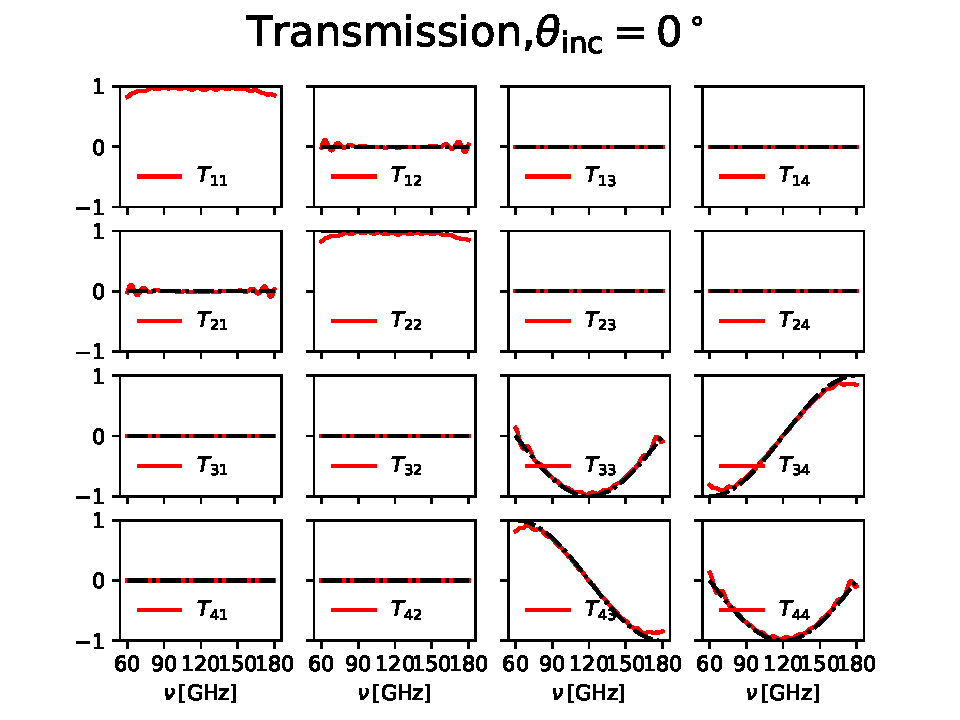
\includegraphics[0.5\linewidth]{figures/1layer_AHWP_120.pdf}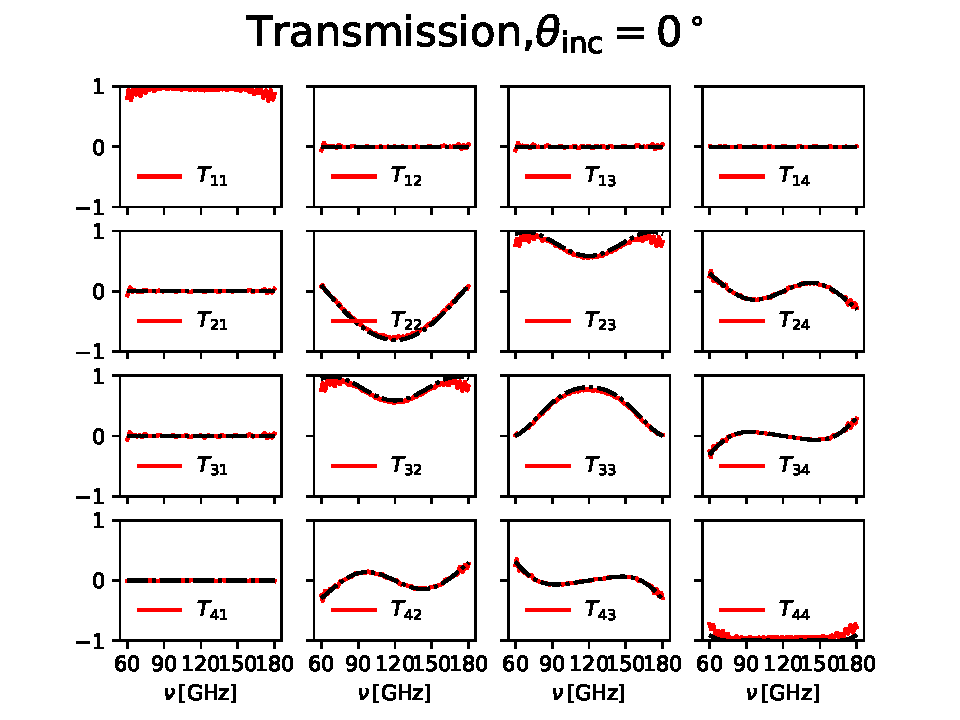
\includegraphics[0.5\linewidth]{figures/3layer_AHWP_120.pdf}
\end{center}
\caption{Mueller matrix elements $M_{ij}$ for a single-layer HWP (left panel) and a three-layer AHWP (right panel) as a function of the frequency of the incident radiation. Each layer is a made of Sapphire crystal and it is optimized for a central frequency of $120\,\mathrm{GHz}$. The AHWP is optimized to cover the broad-band range including the $90\,\mathrm{GHz}$ and $150\,\mathrm{GHz}$ frequency bands. The behaviour of $M_{ij}$ with the frequency for the single-layer HWP agrees with the description in eq.~(\ref{eq:Mueller_Matrix}). The behaviour of $M_{ij}$ for the AHWP is more complicated and agrees with the combination of three Mueller matrices as in eq.~(\ref{eq:Mueller_Matrix}) and rotated with respect to each other. Further details are provided in Sec.~\ref{subsec:modeff}. In both panels, the black dashed-dotted lines correspond to the elements of an ideal HWP.}\label{fig:Mueller_elements}
\end{figure}

For an achromatic HWP, made of stacks of birifringent material, the Mueller matrix presents further non-zero terms with respect to the ones in eq.\,(\ref{eq:Mueller_Matrix}), see Sec.\,\ref{subsec:modeff}. The right panel of Fig.~\ref{fig:Mueller_elements} shows the Mueller matrix elements $M_{ij}$ for a three-layer AHWP as a function of the frequency of the incoming radiation. The presence of additional non-zero elements with respect to the single-layer HWP is clearly visible. 

The HWP optical action creates a non zero $c$ and $s$ terms. Because this does not depend on the direction of the incoming radiation (upwards or downwards), the HWP Mueller matrix has the same shape, eq.\,(\ref{eq:Mueller_Matrix}), both in transmission and in reflection; the value of the corresponding Mueller matrix components changes according to the amplitudes of the electric field transmitted and reflected by the HWP.








